\documentclass{article}
\usepackage[utf8]{inputenc}

\usepackage{amsthm,amssymb,amsmath}
\usepackage{graphicx}
\usepackage{float}

\newcommand{\NN}{\mathbb{N}}
\newcommand{\ZZ}{\mathbb{Z}}
\newcommand{\RR}{\mathbb{R}}
\newcommand{\QQ}{\mathbb{Q}}
\newcommand{\CC}{\mathbb{C}}

\title{AERO7970 - Trajectory Optimiztion \\ {\small Project 03}}
\author{Matt Boler}
\date{\today}

\begin{document}

\maketitle

\begin{abstract}
  This report details the implementation of a fuel-optimal close-proximity rendezvous maneuver with obstacle avoidance.
  The solution was implemented in \texttt{Matlab} usingthe built-in \texttt{solve} function.
  Included are performance comparisons and the resulting trajectories and control inputs.
\end{abstract}

%%
\section{Problem Modeling}

We are given the optimization problem from Project 1 with the added goal of avoiding the obstacle defined by
\begin{itemize}
  \item $-0.6km \leq x \leq -0.5km$
  \item $0.45km \leq y \leq 0.55km$
  \item $-0.01km \leq z \leq 0.01km$
\end{itemize}

We use the same techniques as before (introducing a variable to bound the L1 norm, discretizing the dynamics, etc).
In addition, we use the Big-M technique to handle the nonfeasible region of the obstacle by introducing variables $Z$ with constraints:
\begin{align*}
  -X(t) &\leq -X_{max} + M * Z_{x1}(t) \\
  -Y(t) &\leq -Y_{max} + M * Z_{y1}(t) \\
  -Z(t) &\leq -Z_{max} + M * Z_{z1}(t) \\
  X(t) &\leq X_{min} + M * Z_{x2}(t) \\
  Y(t) &\leq Y_{min} + M * Z_{y2}(t) \\
  Z(t) &\leq Z_{min} + M * Z_{z2}(t)
\end{align*}


\section{Results}

The problem was solved in \texttt{Matlab} using the \texttt{intlinprog} solver.
The resulting trajectory is presented below alongside the original trajectory for comparison.
It is worth noting that in problems of this form, while the individual discretization points may avoid the obstacle, actually following the solved trajectory may cause the chaser to collide with the obstacle.
This is due to the discretization of the trajectory, which causes constraints to only be evaluated at select points.
The trajectory between the discretization points can intersect the obstacle without violating constraints.

\begin{figure}[H]
  \centering
  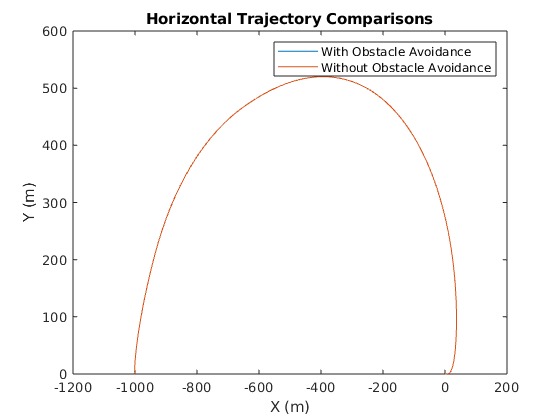
\includegraphics[width=0.7\textwidth]{images/horizontal_traj.png}
  \caption{Overhead view of generated trajectories}
  \label{fig:overhead-trajectories}
\end{figure}

\begin{figure}[H]
  \centering
  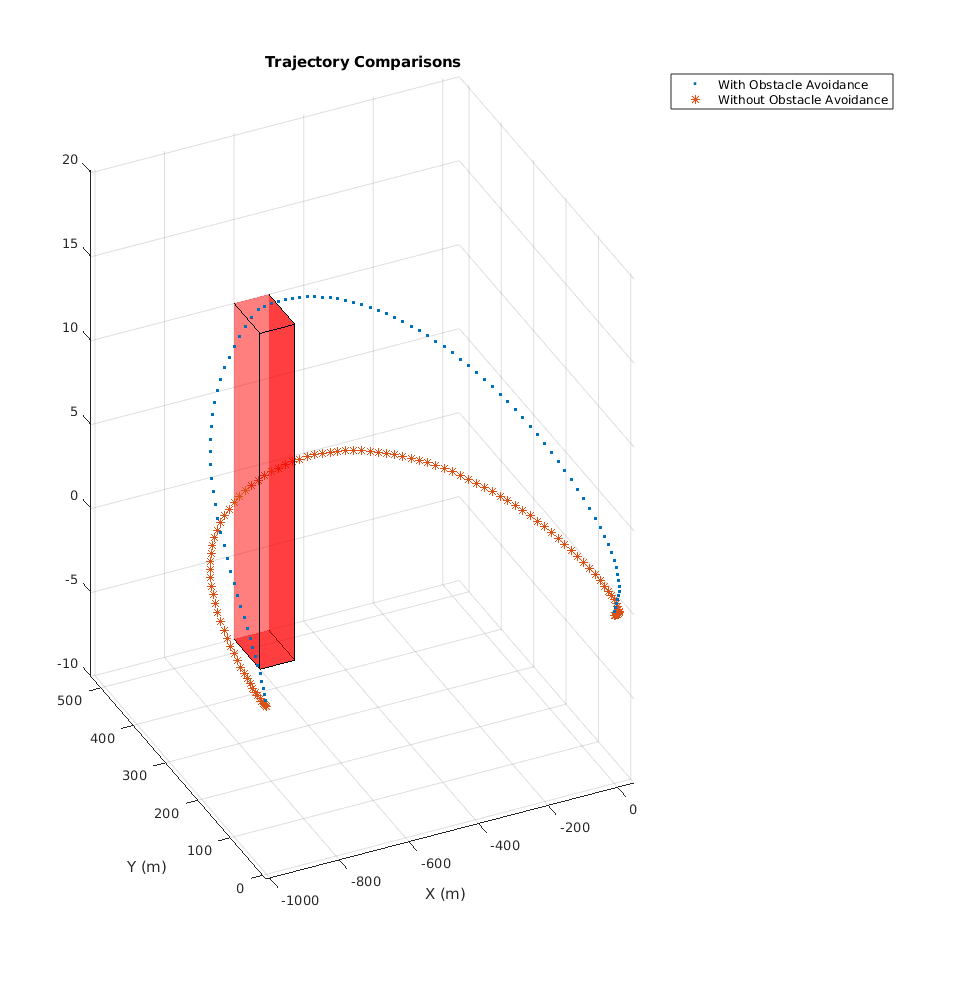
\includegraphics[width=0.7\textwidth]{images/traj.png}
  \caption{3d view of generated trajectories}
  \label{fig:trajectories}
\end{figure}

\begin{figure}[H]
  \centering
  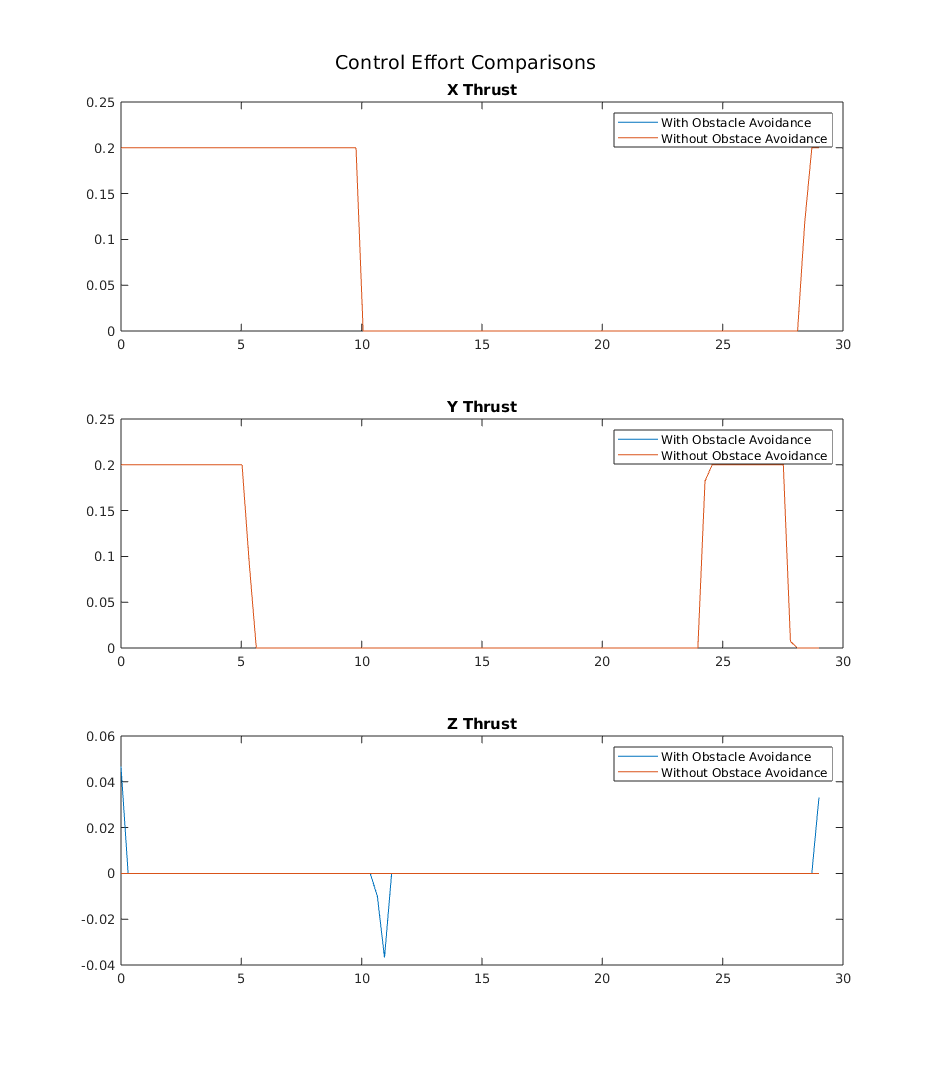
\includegraphics[width=0.7\textwidth]{images/control.png}
  \caption{Optimal control efforts}
  \label{fig:controls}
\end{figure}

Afterwards, the same problem was solved with the modificaion of $Y_{min} = 0.35km$.
This resulted in a very similar optimal trajectory, except that the chaser now flies under the obstacle instead of over it.
The results are shown below.

\begin{figure}[H]
  \centering
  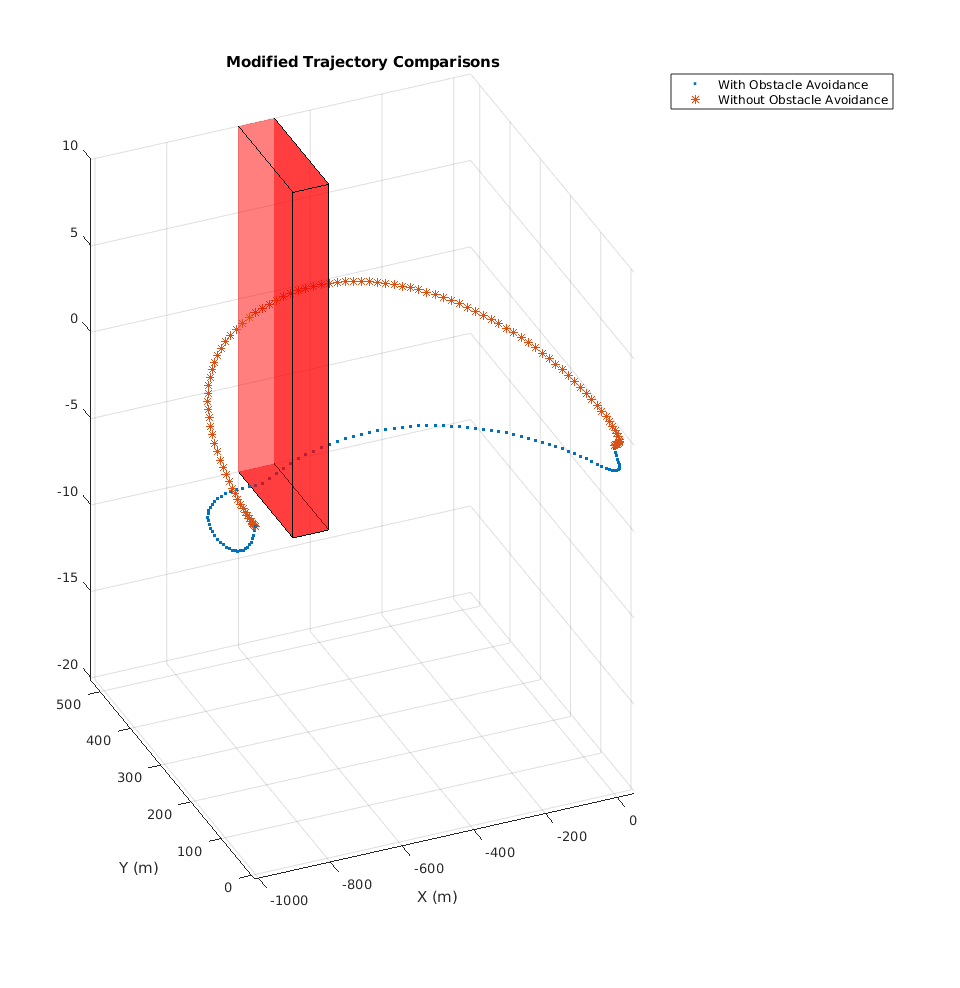
\includegraphics[width=0.7\textwidth]{images/traj_mod.png}
  \caption{3d view of generated trajectories}
  \label{fig:trajectories-modified}
\end{figure}

\begin{figure}[H]
  \centering
  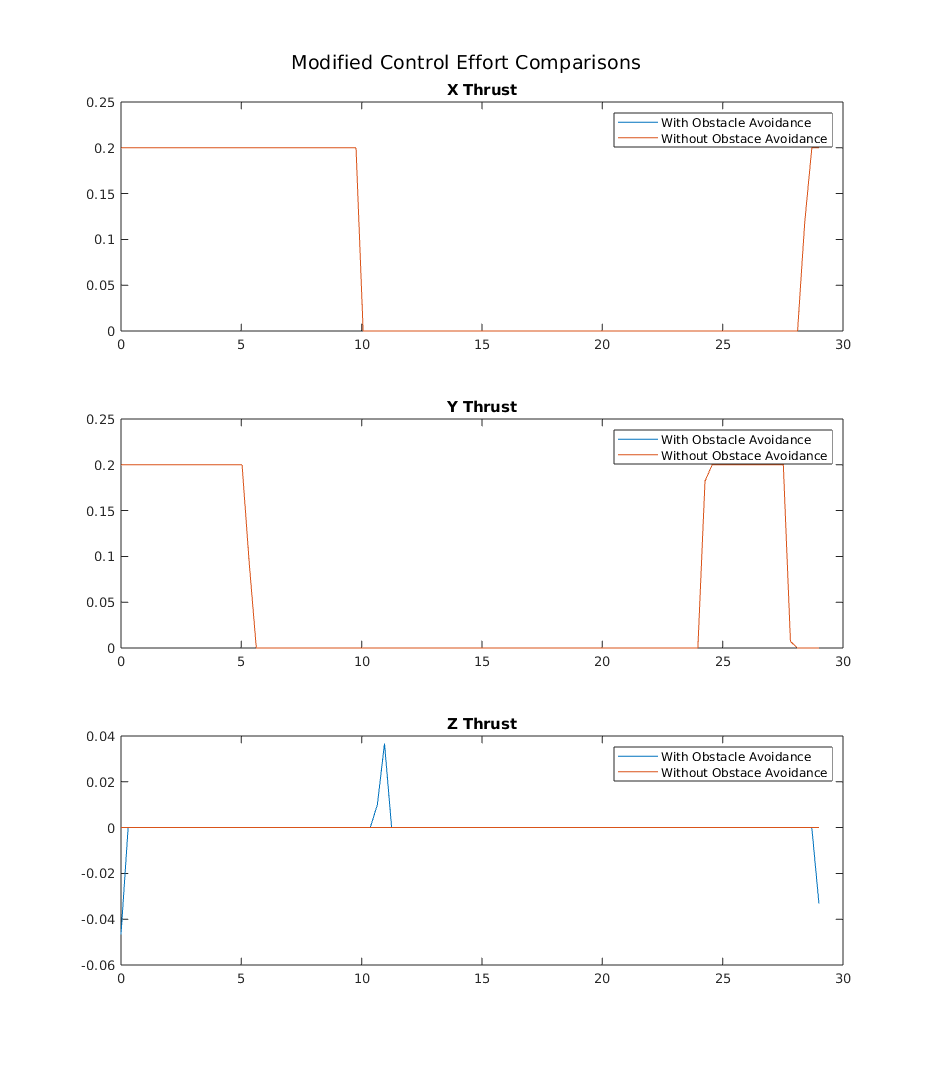
\includegraphics[width=0.7\textwidth]{images/control_mod.png}
  \caption{Optimal control efforts}
  \label{fig:controls-modified}
\end{figure}

\section*{Conclusion}

This problem did not have any major challenges, as it was a simple modification of an earlier problem.
The main thing I learned is that integrating square (or generally convex?) state constraints is simple and fast, which should help me down the road in my research.
I spent approximately 3 hours on this project.
\end{document}
